
\section{Manual Patches}

An image can have multiple discriminating patches. As shown in Figure \ref{fig:manual_patch}, some patches are highly noticeably discriminating such an open mouth and raised eyebrows in �surprise� expression or a wrinkled glabella (area between eyes) in �disgust� expression. All the emotions can be distinguised by one or more such patches. Hence these patches can be the best approximation of most discriminating patches. Hence, they make a good basis for testing the algorithm.  We identified four such patches, that 2 patches for eyes and one each for mouth and glabella.  Histogram of oriented gradients, which is used for feature extraction, works on edge detection. Clearly, these four patches have more edges than rest of the face (such as cheeks or forehead).

\begin{figure}
\centering
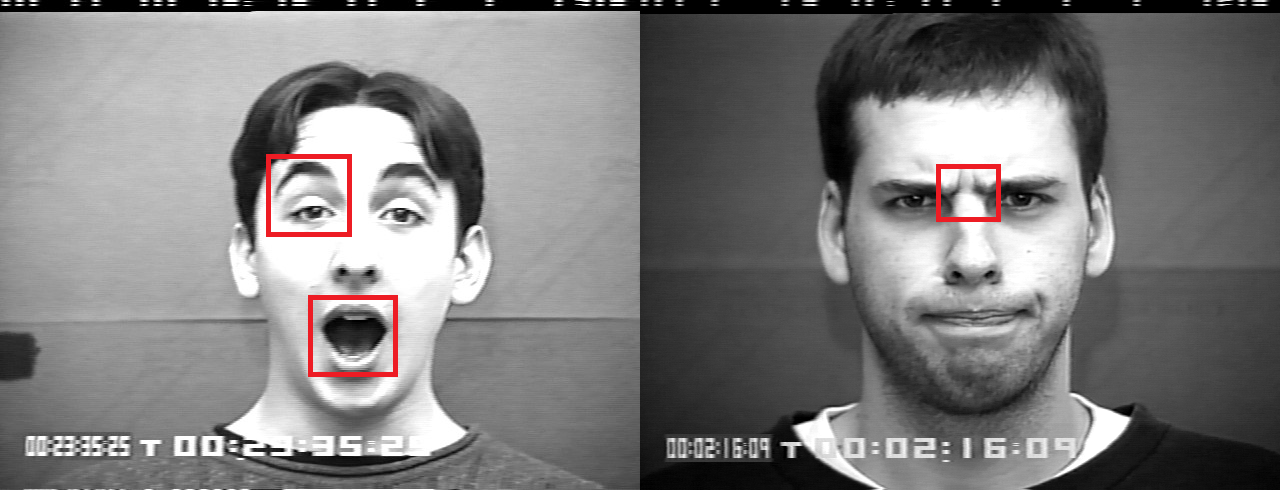
\includegraphics[width=300pt]{manual_patch.png}
  \caption{Noticeably discriminating patches}
  \label{fig:manual_patch}
\end{figure}

We extracted them manually and resized them to 36*36 pixels, 64*64 pixels and 96*96 pixels. It was ensured that extracted images of same patch are consistent with each other in terms feature content of the patch. For example, in case of mouth patches, it was ensured that the boundaries of the patch touch the edges of lips in all mouth patches.  It is very important that the patches are consistent and optimal otherwise the results can be poor. This is reflected from Table \ref{table:predict_unaliged_surprise} and Table \ref{table:predict_unaliged_fear}.

\begin{table*}
\centering
\newcommand{\tabincell}[2]{\begin{tabular}{@{}#1@{}}#2\end{tabular}}
\caption{Predicting the unaligned patches from surprise emotion}
\label{table:predict_unaliged_surprise}

\begin{tabular}{| c | c | c | c | c |}
\hline
Patches & Mouth & Left-eye  & Right-eye & \tabincell{c}{Part \\ between eyes}  \\
\hline
1 & sadness & disgust & surprise & fear \\
2 & sadness & fear & disgust & fear \\
3 & neutral & surprise & happy & disgust \\
4 & neutral & disgust & happy & surprise \\
5 & disgust & fear & disgust & fear \\
6 & surprise & fear & sadness & disgust \\
7 & surprise & surprise & sadness & disgust \\
8 & disgust & sadness & disgust & fear \\
9 & surprise & angry & surprise & surprise \\
10 & fear & surprise & disgust & surprise \\
11 & surprise & angry & sadness & fear \\
12 & surprise & angry & disgust & disgust \\
13 & fear & surprise & disgust & disgust \\
14 & surprise & fear & surprise & disgust \\
15 & surprise & surprise & fear & fear \\

\hline
\end{tabular}
\end{table*}


\begin{table*}
\centering
\newcommand{\tabincell}[2]{\begin{tabular}{@{}#1@{}}#2\end{tabular}}
\caption{Predicting the unaligned patches from fear emotion}
\label{table:predict_unaliged_fear}

\begin{tabular}{| c | c | c | c | c |}
\hline
Patches & Mouth &  Left-eye  & Right-eye & \tabincell{c}{Part \\ between eyes} \\
\hline
1 & happy & fear & fear & disgust \\
2 & happy & disgust & fear & fear \\
3 & contempt & surprise & contempt & fear \\
4 & contempt & disgust & contempt & disgust \\
5 & fear & disgust & disgust & fear \\
6 & fear & fear & sadness & angry \\
7 & disgust & sadness & sadness & surprise \\
8 & fear & disgust & disgust & angry \\
9 & fear & disgust & disgust & fear \\
10 & fear & surprise & disgust & disgust \\
11 & fear & surprise & surprise & fear \\
12 & contempt & fear & disgust & fear \\
13 & fear & disgust & disgust & surprise \\
14 & contempt & disgust & fear & disgust \\
15 & happy & fear & fear & disgust \\
\hline
\end{tabular}
\end{table*}



